% Что пишем в программную реализацию?

% \begin{enumerate}
%   \item Раскрываем, какой язык программирования используем
%   \item Раскрываем какие библиотеки используем
%   \item Раскрываем поэтапно по шагам
% \end{enumerate}

% На каком языке программировании написано
\subsection*{Технология}
Описанная модель реализована на языке программирования Python. Реализация сочетает достоинства применения как парадигмы ООП, так и функционального программирования за счет активного использования лямбда-выражений.

% Какую библиотеку использовали
Для реализации на языке программирования был использован внешний модуль pyomo. В части решаемой задачи этот модуль был задействован для построения математической модели и взаимодействия с решателями. Построение математической модели заключалось в динамической генерации переменных и ограничений. Взаимодействие с решателями - вызов их из переменных окружения среды, задание входных аргументов для их работы и считывание результатов вычислений.

\subsection*{Умножение матриц бинарных параметров}
Функция перемножения бинарных матриц используется как альтернатива обычному перемножению для исключения в моделе нелинейности. Перемножая матрицы обычным способом появляются нелинейные выражения. Наличие нелинейности в моделе приведет к значительному усложенению ее решения и невозможности ее решения большинством программных решателей.

С целью невелирования этого обстоятельства целевая функция в частности и модель в целом должны быть переработаны. Переработка базируется на том обстоятельстве, что перемножаются не матрицы в общем виде, а матрицы именно бинарных параметров. Как известно, перемножение матриц заключается в суммировании произведений соответвтующих элементов двух матриц. Каждое произведение элементов $x \cdot y$, где $x$ и $y$ значения бинарных параметров, может быть заменено дополнительной переменной $f$, значение которой должно удовлетворять следующим ограничениям:
\begin{center}
  $
  \begin{cases}
    x + y <= f + 1 & \quad \text{в таблице \ref{tab:fbm} имеет обозначение } f_{1} \\
    f <= x     & \quad \text{в таблице \ref{tab:fbm} имеет обозначение } f_{2} \\
    f <= y     & \quad \text{в таблице \ref{tab:fbm} имеет обозначение } f_{3}
  \end{cases}
  $
\end{center}
Демонстрация робастности ограничений приведена в таблице \ref{tab:fbm}:
\begin{longtable}{|c|c|c|c|c|c|c|}
  \caption{Робастность ограничений $f_{bm}$}
  \label{tab:fbm}\\   
  \hline
  $x$ & $y$ & $f$ & $f_{1}$ & $f_{2}$ & $f_{3}$ & $f_{1} \vee f_{2} \vee f_{3}$ \\
  \endfirsthead
  $x$ & $y$ & $f$ & $f_{1}$ & $f_{2}$ & $f_{3}$ & $f_{1} \vee f_{2} \vee f_{3}$ \\
  \endhead
  \endfoot
  \hline
  0 & 0 & 0 & true  & true  & true  & true \\
  \hline
  0 & 0 & 1 & true  & false & false & false \\
  \hline
  0 & 1 & 0 & true  & true  & true  & true \\
  \hline
  0 & 1 & 1 & true  & false & true  & false \\
  \hline
  1 & 0 & 0 & true  & true  & true  & true \\
  \hline
  1 & 0 & 1 & true  & true  & false & false \\
  \hline
  1 & 1 & 0 & false & true  & true  & false \\
  \hline
  1 & 1 & 1 & true  & true  & true  & true \\
  \hline
\end{longtable}

\subsection*{Функция определения вхождения}
Функция определения вхождения $f_{in}$ применяется с целью преобразования большего или равного $0$ входного параметра в бинарное значение.

Функцию $f_{in}$ следует представить в виде переменных и ограничений в модели. Для этого используется метод big M. Этот метод предписывает заведение в моделе дополнительной бинарной переменной $f$, значение которой должно удовлетворять следующим ограничениям:
\begin{center}
  $
  \begin{cases}
    f < x + 1 & \quad \text{в таблице \ref{tab:fin} имеет обозначение } f_{1} \\
    x \le M \cdot f & \quad \text{в таблице \ref{tab:fin} имеет обозначение } f_{2}
  \end{cases}
  $
\end{center}

Здесь $M$ - условно большое число. Демонстрация робастности ограничений приведена в таблице \ref{tab:fin}:
\begin{longtable}{|c|c|c|c|c|}
  \caption{Робастность ограничений $f_{in}$}
  \label{tab:fin}\\   
  \hline
  $x$ & $f$ & $f_{1}$ & $f_{2}$ & $f_{1} \vee f_{2}$ \\
  \endfirsthead
  $x$ & $f$ & $f_{1}$ & $f_{2}$ & $f_{1} \vee f_{2}$ \\
  \endhead
  \endfoot
  \hline
  0              & 0 & true  & true  & true \\
  \hline
  0              & 1 & false & true  & false \\
  \hline
  (0 ; 1)        & 0 & true  & false & false \\
  \hline
  (0 ; 1)        & 1 & true  & true  & true \\
  \hline
  1              & 0 & true  & false & false \\
  \hline
  1              & 1 & true  & true  & true \\
  \hline
  (1 ; $\infty$) & 0 & true  & false & false \\
  \hline
  (1 ; $\infty$) & 1 & true  & true  & true \\
  \hline
\end{longtable}

\subsection*{Функция определения реализованности}
Функция определения реализованности $f_{im}$ применяется с целью преобразования большего или равного $0$ входного параметра в бинарное значение.

Функцию $f_{im}$ следует представить в виде переменных и ограничений в моделе. Для этого используется ранее упомянутый метод big M. Следуя ему, ограничения на значение дополнительной бинарной переменной $f$ следующие:
\begin{center}
  $
  \begin{cases}
    x \geq f & \quad \text{в таблице \ref{tab:fim} имеет обозначение } f_{1} \\
    x < M \cdot f + 1 & \quad \text{в таблице \ref{tab:fim} имеет обозначение } f_{2}
  \end{cases}
  $
\end{center}

Демонстрация робастности ограничений приведена в таблице \ref{tab:fim}:
\begin{longtable}{|c|c|c|c|c|}
  \caption{Робастность ограничений $f_{im}$}
  \label{tab:fim}\\   
  \hline
  $x$ & $f$ & $f_{1}$ & $f_{2}$ & $f_{1} \vee f_{2}$ \\
  \endfirsthead
  $x$ & $f$ & $f_{1}$ & $f_{2}$ & $f_{1} \vee f_{2}$ \\
  \endhead
  \endfoot
  \hline
  0              & 0 & true  & true  & true \\
  \hline
  0              & 1 & false & true  & false \\
  \hline
  (0 ; 1)        & 0 & true  & true  & true \\
  \hline
  (0 ; 1)        & 1 & false & true  & false \\
  \hline
  1              & 0 & true  & false & false \\
  \hline
  1              & 1 & true  & true  & true \\
  \hline
  (1 ; $\infty$) & 0 & true  & false & false \\
  \hline
  (1 ; $\infty$) & 1 & true  & true  & true \\
  \hline
\end{longtable}

% Про ограничения и появление 1 / M
\subsection*{Описание строгих неравенств}
Часть ограничений модели описана при помощи знаков строгого неравенсва. Модуль pyomo предписывает задание ограничений на значения параметра при помощи только нестрогих неравенств. С целью невелирования данного обстоятельства используется константа равная $1 / M$ - условно малое число. Тогда ограничение модели вида $x < y$ будет описано как $x + 1 / M \le y$.

% Раскрыть применение матрешки
\subsection*{Организация кода}
С целью понижения когнитивной сложности применяемого решения и достижения управляемости поведением каждой отдельной единицы функционала весь код разбит на обособленные модули, представленные в виде классов языка программирования Python.

Компоновка их друг с другом, последовательное разрешение зависимостей происходит в едином месте - в главной функции программы. В такой схеме отсутствуют передача локальных неуправляемых параметров по цепочке вызовов в иерархии функций, а каждая отдельная единица функционала работает в своем информационном окружении.

% Привести диаграмму вызовов или uml-диаграмму
Диаграмма классов приведена на рисунке \ref{fig:uml}.

% Рисунок uml-диагараммы
\begin{figure}[H]
    \centering
    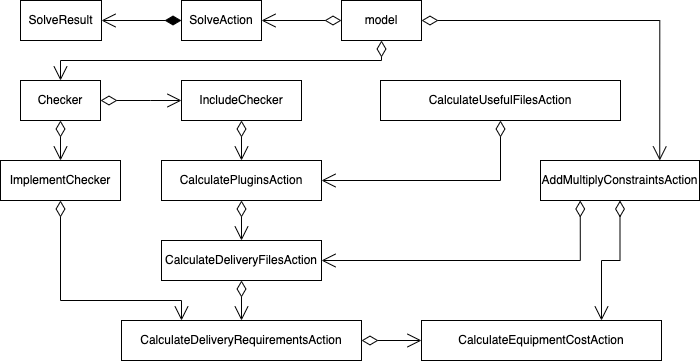
\includegraphics[width=1\textwidth]{uml}
    \caption{Диаграмма классов}
    \label{fig:uml}
\end{figure}
